\subsection{Qualitative results}
\label{sec:gallery}
Figure~\ref{fig:worked} walks through the pipeline on one synthetic plate. Figures~\ref{fig:gallp}
and~\ref{fig:galcc} show held-out real plates. The rows are chosen by rule from the
experiment-5 results, not by hand: the largest accepted gains, typical accepted gains, the worst and
the best refused case, and the worst accepted case.

\begin{figure}[h]
\centering
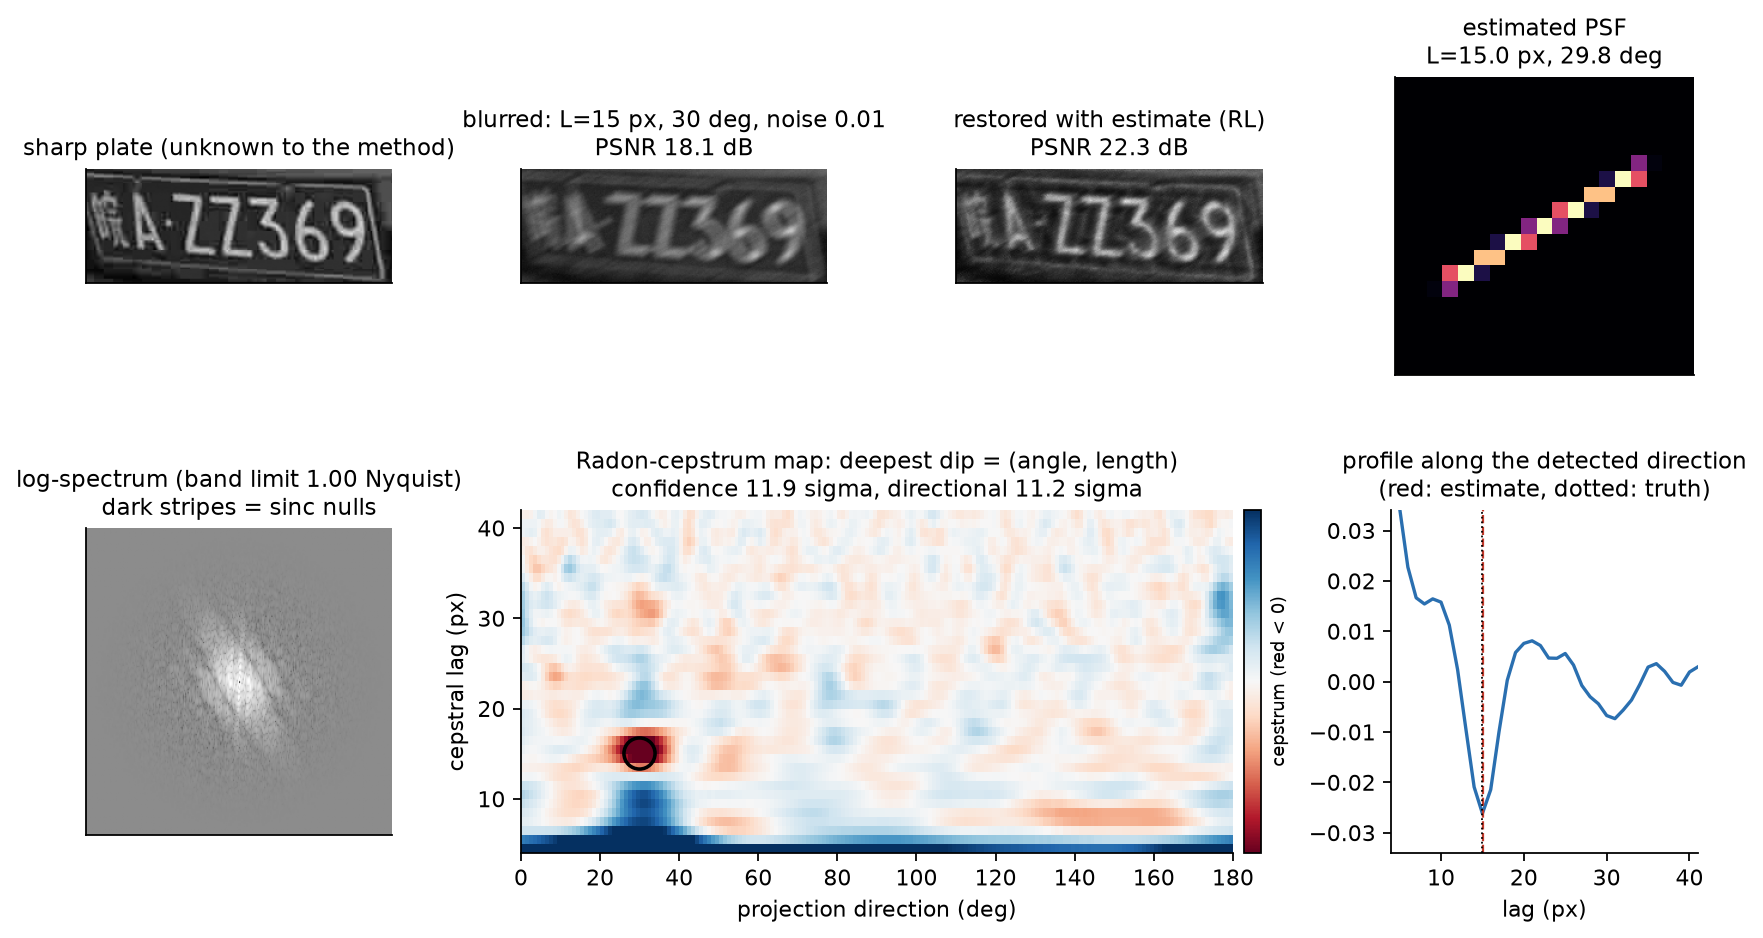
\includegraphics[width=\textwidth]{07_worked_example.png}
\caption{Worked example ($L=15$\,px, $30^\circ$, $\sigma=0.01$). The log-spectrum shows the dark
null stripes; the Radon--cepstrum map has a single deep dip at the true (angle, length); the
estimate is within $0.2^\circ$ and $0.1$\,px.}
\label{fig:worked}
\end{figure}

\begin{figure}[p]
\centering
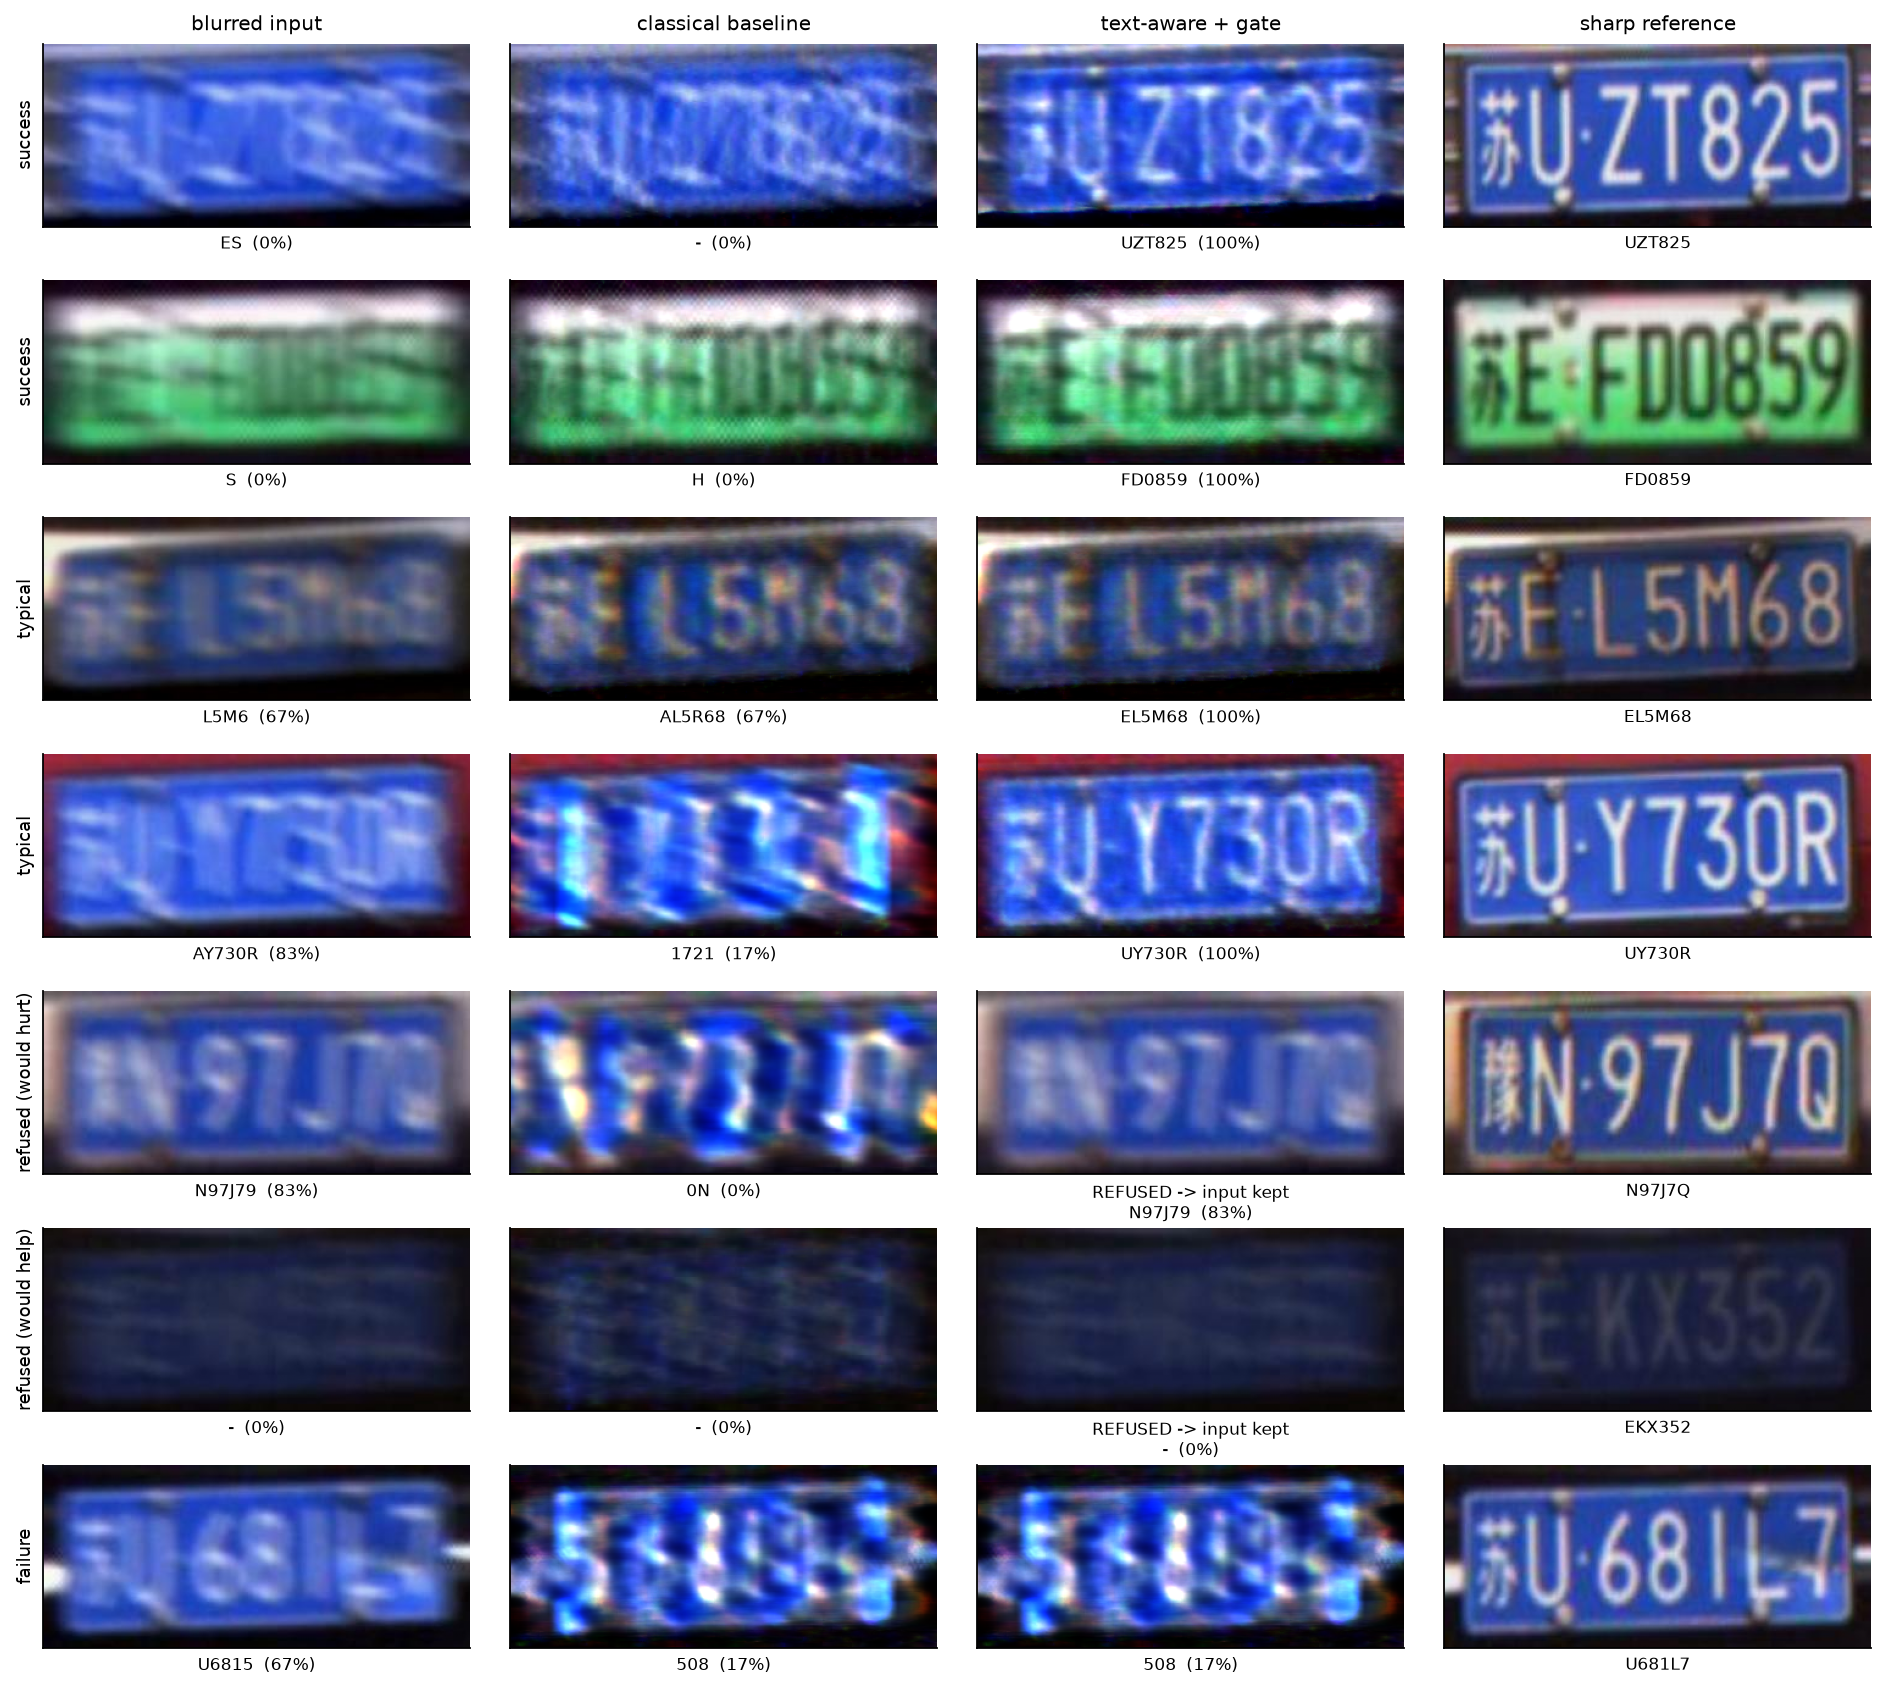
\includegraphics[width=0.93\textwidth]{07_gallery_lpblur.png}
\caption{LPBlur test plates (OCR reading and character accuracy under each image). The classical
baseline often produces strong ringing (rows 4--5): its full-band estimate is wrong. The gate refuses
a case that would have been destroyed (row 5) and, at the price of a missed improvement, a very dark
plate (row 6). Row 7 is a failure the gate let through.}
\label{fig:gallp}
\end{figure}

\begin{figure}[p]
\centering
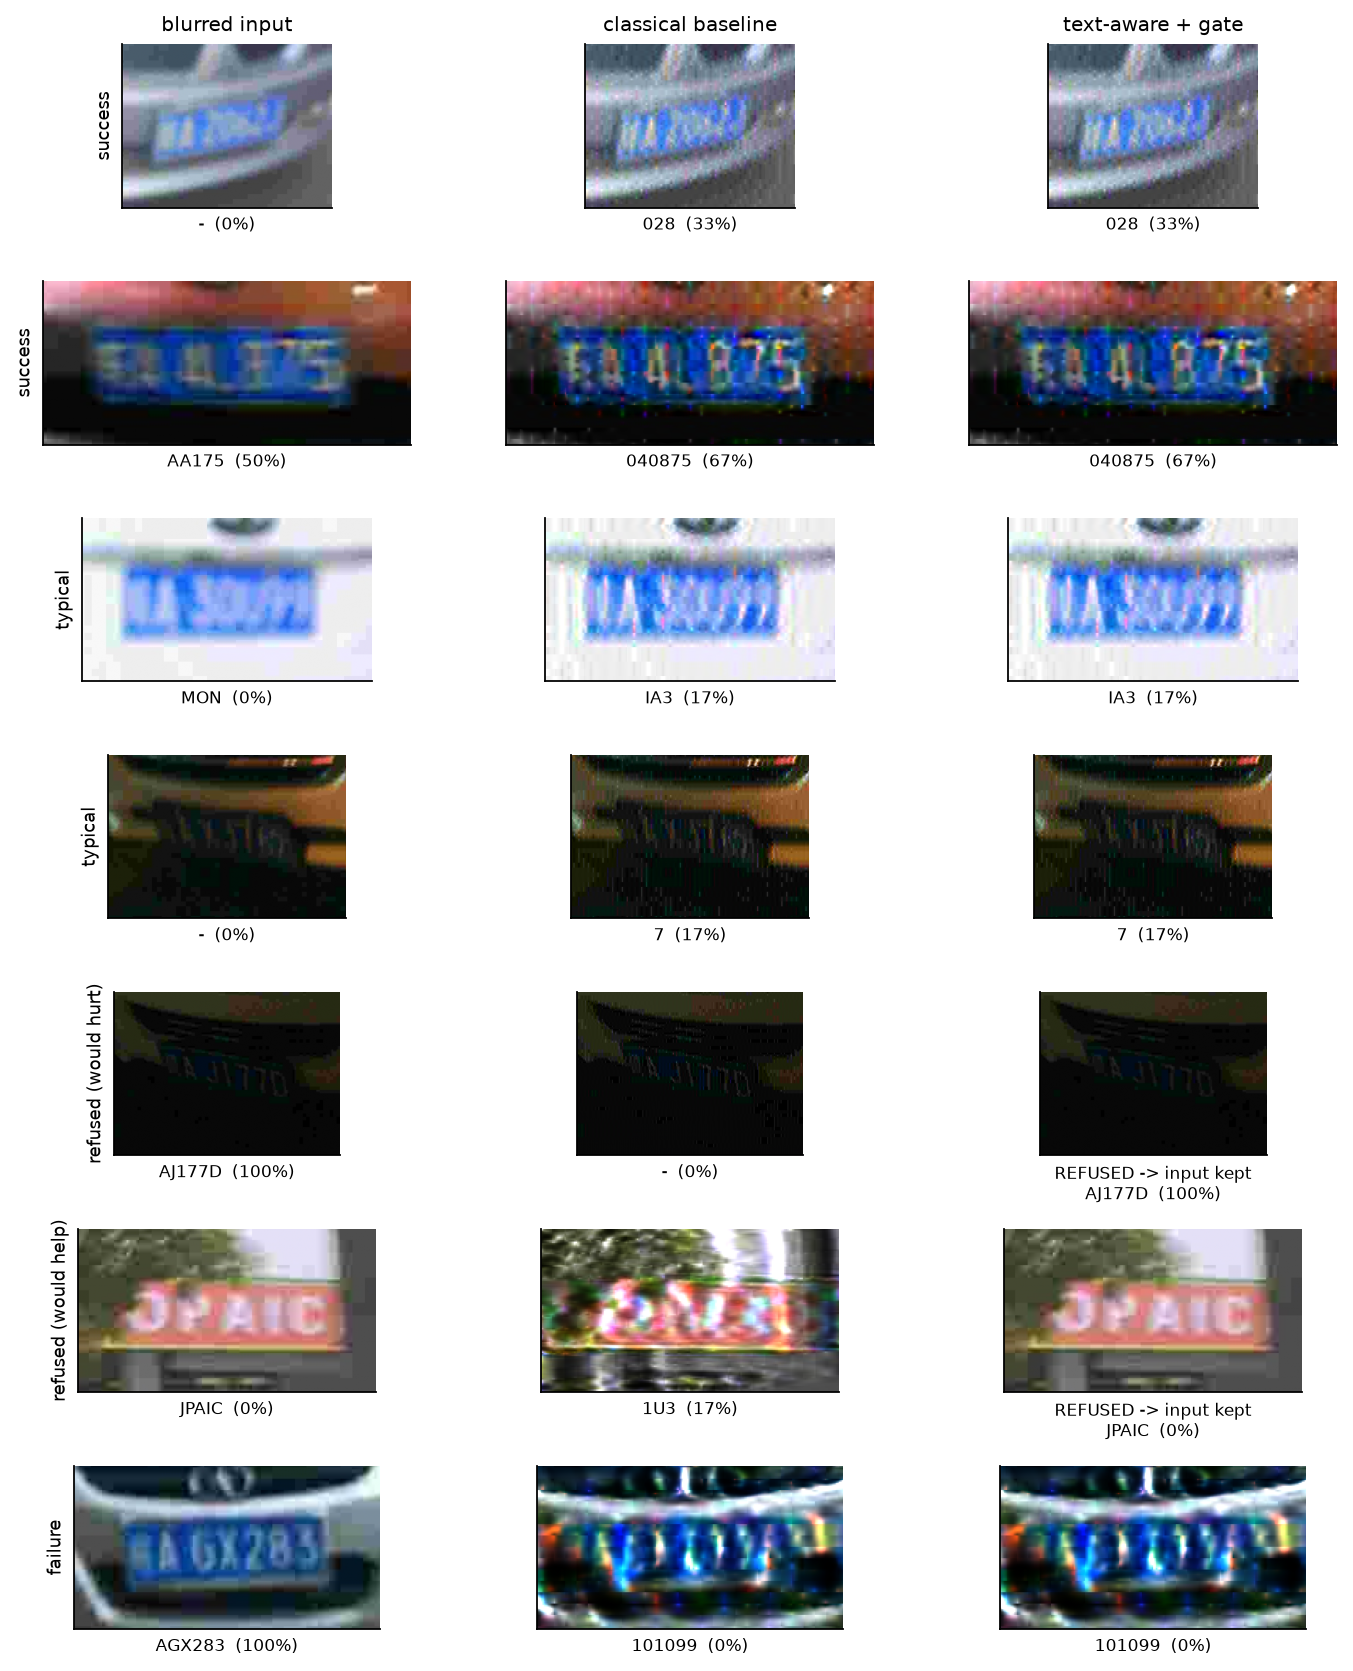
\includegraphics[width=0.93\textwidth]{07_gallery_ccpd.png}
\caption{CCPD-Blur test plates. Most of this blur is not linear motion; the few accepted restorations
help modestly, and the gate's refusals keep readable plates readable.}
\label{fig:galcc}
\end{figure}
